\RequirePackage[herbstlich]{TUcolor}
\documentclass[compress]{beamer}
\usepackage[utf8]{inputenc}
\usepackage{listings}
\usepackage{eurosym}
\usepackage{bibgerm}
\usepackage{wasysym}
\usepackage[style=alphabetic]{biblatex}
\usepackage[orientation=landscape,size=custom,width=16,height=12,scale=0.55]{beamerposter}
\title[MicroMoody]
	{MicroMoody-Update\\\small Status und Erkenntnisse}
\author{derf}
\institute{Chaosdorf}
\date{\today}

\usetheme{Warsaw}
\setbeamertemplate{footline}[frame number]
\setbeamertemplate{navigation symbols}{}
%\setbeamertemplate{navigation symbols}{\insertframenumber{} / \inserttotalframenumber\hspace*{1ex}}
%\setbeamercolor{section in head/foot}{fg=black,bg=TUDogreen}
%\setbeamercolor{subsection in head/foot}{fg=black,bg=TUDogreen}
%\setbeamercolor{itemize item}{bg=red}
%\setbeamercolor{bulletpoint}{bg=red}
%
\setbeamercolor{palette primary}{fg=white,bg=TUDogreen} % changed this
\setbeamercolor{local structure}{fg=TUDogreen}
%\setbeamercolor{palette secondary}{fg=yellow,bg=red} % changed this
%\setbeamercolor{palette tertiary}{fg=red,bg=yellow} % changed this

\renewcommand{\familydefault}{\sfdefault}
\renewcommand{\footnoterule}{}

\lstset{numbers=left}

\begin{document}

\begin{frame}
	\titlepage
\end{frame}

\section{MicroMoody}
\begin{frame}{Wat?}
\begin{columns}
\column{.5\textwidth}
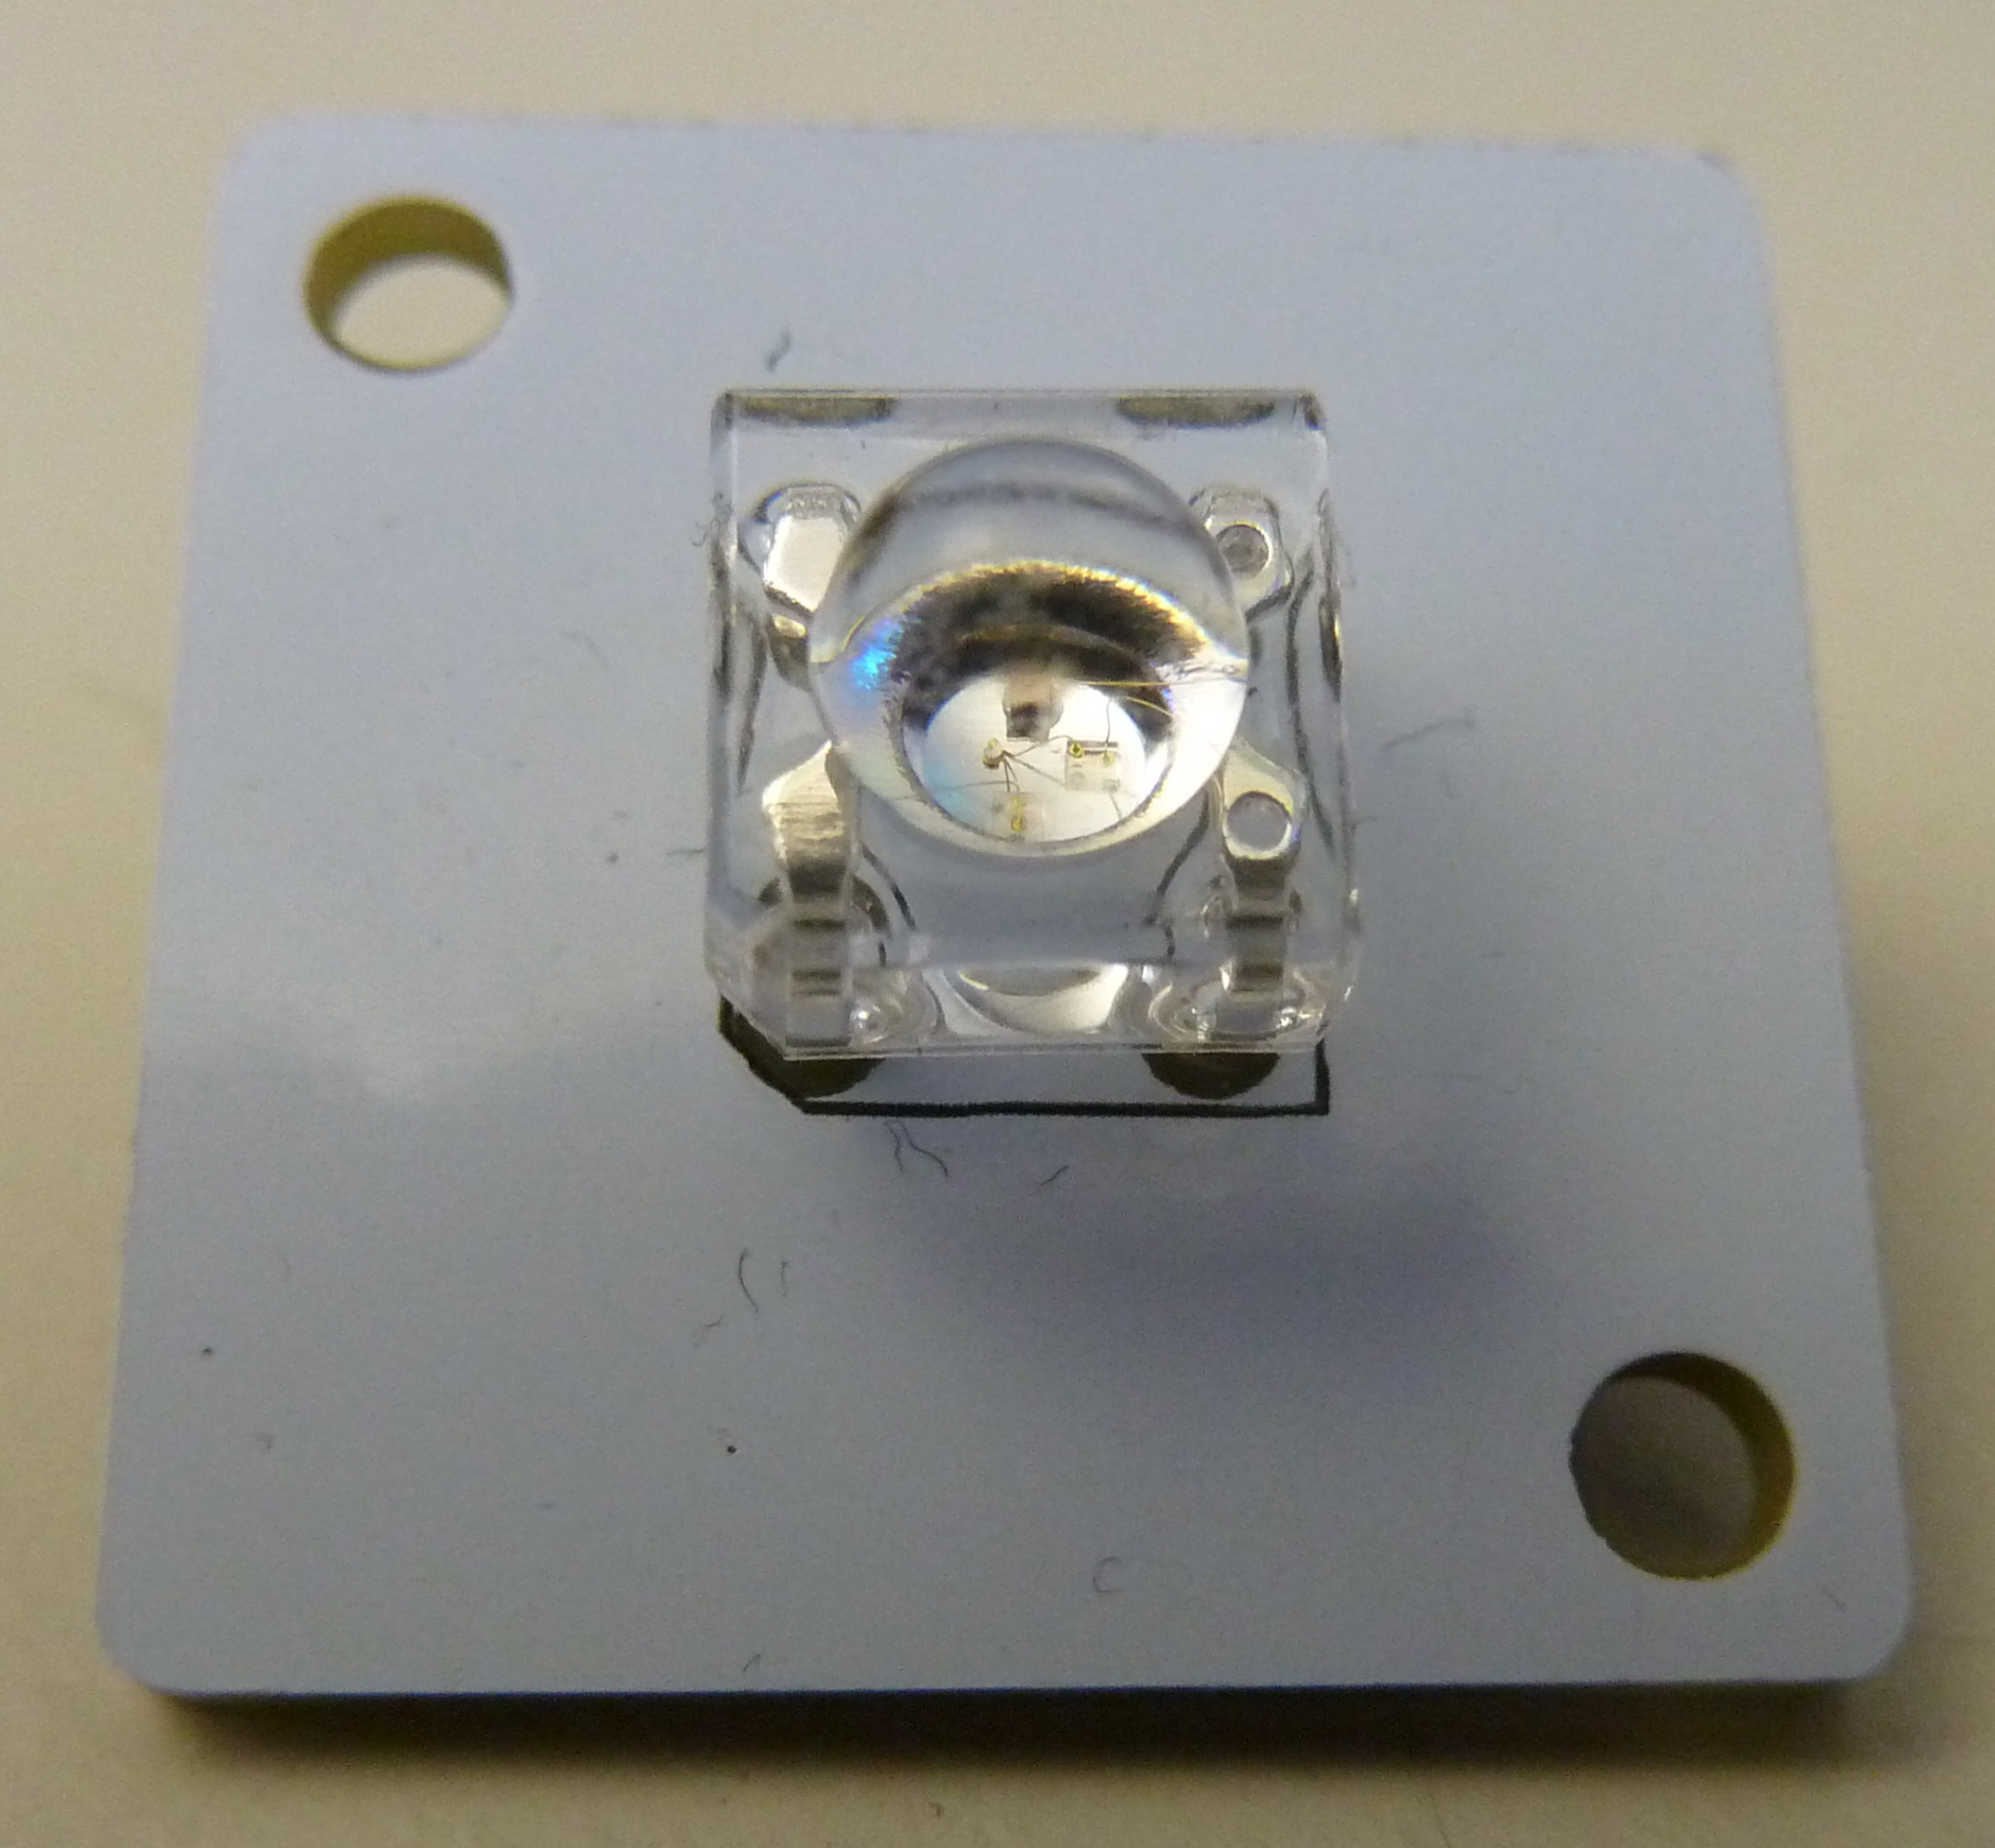
\includegraphics[width=\textwidth]{micromoody_front.jpg}
\column{.5\textwidth}
\begin{itemize}
\item<2-> AVR (ATTiny85) + RGB-LED\\
(furchtbar hell)
\item<3-> kein USB, dafür I$^2$C\\
$\to$ Bus-System
\item<4-> Wenig Bauteile\\
(Materialkosten $< 5$ \euro)
\item<5-> Selbstverständlich:\\
Ein Produkt des RaumZeitLabor
\end{itemize}
\end{columns}
\end{frame}

\begin{frame}{Dat}
\begin{columns}
\column{.5\textwidth}
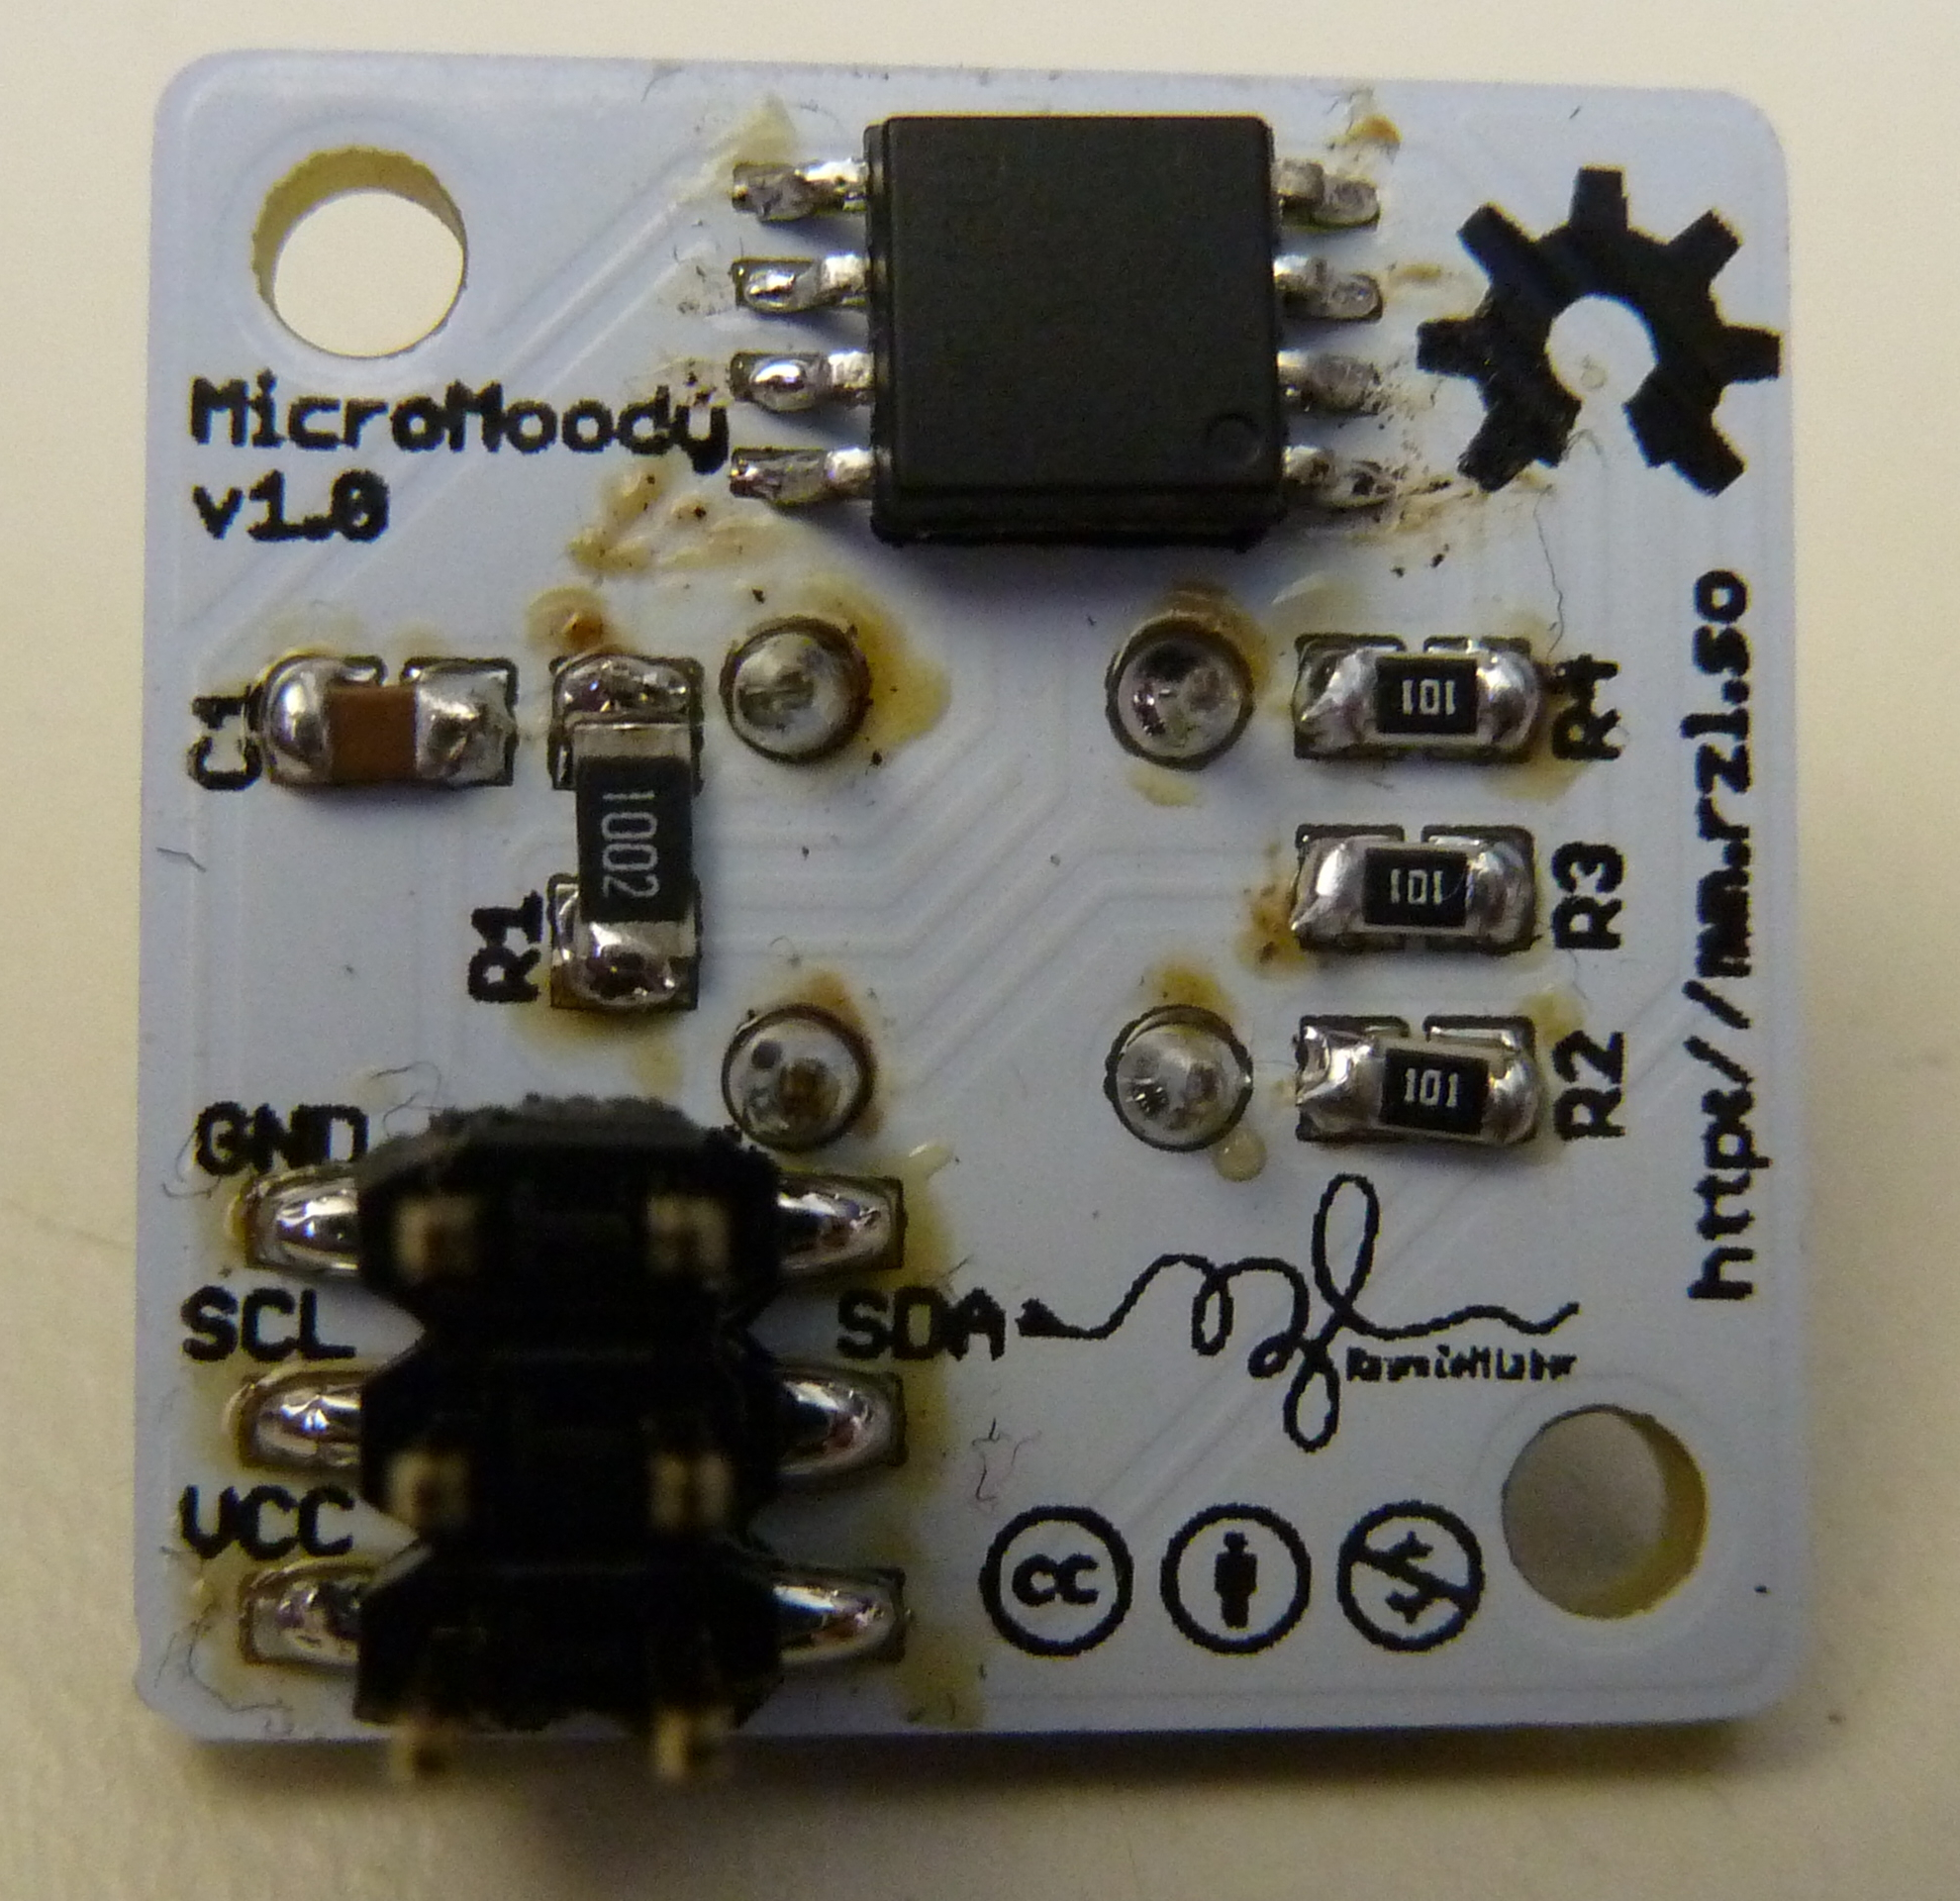
\includegraphics[width=\textwidth]{micromoody_back.jpg}
\column{.5\textwidth}
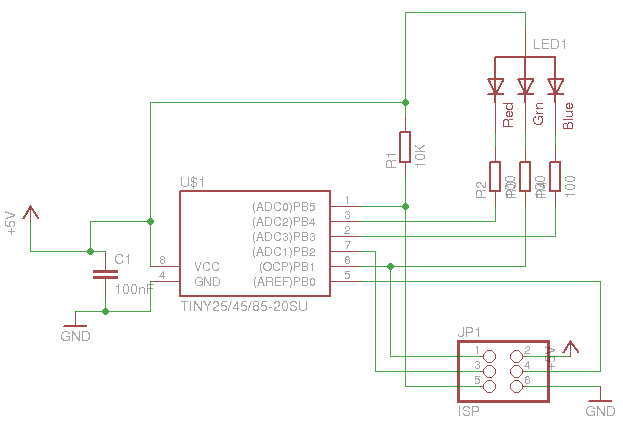
\includegraphics[width=\textwidth]{circuit.png}
\end{columns}
\end{frame}

\subsection{Status}
\begin{frame}{Status}
$\CheckedBox$ Fading (ähnlich dorfmap-RGB-Streifen)\\\pause
$\CheckedBox$ I$^2$C-Fernsteuerung\\\pause
$\CheckedBox$ I$^2$C-Bus (mehrere Moodies)\\\pause
$\Box$ USB $\to$ I$^2$C-Bausatz
\end{frame}

\section{Erkenntnisse}
\begin{frame}{Today I learned...}
\begin{itemize}
\item<1-> Lesen hilft...
\item<2-> Ausreichend Pins sind hilfreich
\item<3-> "`Gute Ideen"' sind gefährlich
\end{itemize}
\end{frame}


\subsection{I$^2$C}
\begin{frame}{I$^2$C | Inter-Integrated Circuits}
\begin{itemize}
\item<1-> I$^2$C: Data und Clock, digital, bidirektional
\item<1-> Bus: Default High (pull-ups), für 0 "`auf Ground ziehen"'\\
{\small (vermeidet Kurzschlüsse)}
\item<2-> S $\to$ Address, R/$\overline{\text{W}}$ $\to$ ACK/NAK
$\to$ (Byte $\to$ ACK/NAK$)^*$\ $\to$ P
\end{itemize}
\uncover<3->{Habe MicroMoody. Möchte testen und fernsteuern.}
\begin{itemize}
\item<3-> Arduino? Lolnope
\item<4-> $\to$ VUSB PowerSwitch: Pins schalten und auslesen\\
{\small (siehe Verstärkersteuerung)}
\item<5-> Software-Pull-Ups sind \textbf{kein} Ersatz für echte
Widerstände
\item<6-> Nach Lesen der Spec: Funktioniert jetzt sogar
\end{itemize}
\end{frame}

\subsection{Pins}
\begin{frame}{ATTiny85}
\begin{columns}
\column{.5\textwidth}
\begin{itemize}
\item<1-> 8 Pins, $6\times$ IO
\item<2-> 3 Pins für LED
\item<3-> $+ 4$ Pins für ISP (davon 2 I$^2$C)
\item<4-> $= 7$ von 6 Pins benötigt
\item<5-> $\Rightarrow$ Doppelbelegung
\end{itemize}
\column{.5\textwidth}
\includegraphics<6->[width=\textwidth]{circuit-err.png}
\end{columns}
\end{frame}

\begin{frame}{Doppelbelegung}
\begin{itemize}
\item<1-> D.h.: \textbf{PB1} (Steuerpin für Grün) mit 6pin-Header verbunden
\item<1-> Nicht für I$^2$C verwendet, aber im Kabel durchkontaktiert
\item<2-> $\to$ Kurzschlüsse, komischer b0rk
\end{itemize}
\uncover<3->{Was tun?}
\begin{itemize}
\item<4-> Designproblem | Nicht in Software lösbar
\item<5-> Workaround: Pin 1 im Flachbandkabel durchschneiden
\item<6-> ... Kabel damit nicht mehr zum Flashen geeignet
\end{itemize}
\end{frame}

\subsection{Gute Ideen}
\begin{frame}{Die Sache mit dem EEPROM}
\ 
{\small (EEPROM: "`Electronically Erasable Programmable Read Only Memory"'\\
| D.h.: SSD/SD-Karte in ganz langsam)}
\begin{itemize}
\item<2-> Idee: Aktuelles Fade-Programm speichern
\item<2-> ... damit es auch ohne Steuerung blinkt wie gewünscht
\item<3-> Eigentlich eine gute Idee?
\end{itemize}
\uncover<4->{"`Warum dauert das Ansteuern so lange?"'}
\begin{itemize}
\item<5-> 7 Statusbytes, EEPROM schreiben: $\approx 2$ms je Byte $\to$ 11ms je Befehl
\item<6-> Auch: Remote Control-Strobo schlecht für Lebensdauer
\item<7-> Jetzt: Modus Speichern über Extrabefehl
\end{itemize}
\end{frame}

\section{tldr}
\begin{frame}{tldr}
\begin{itemize}
\item MicroMoody inzwischen stabil nutzbar
\item<2-> Lesen hilft
\item<2-> Einen Schritt zurückgehen und nochmal denken auch
\item<3-> (und mit anderen Menschen Debuggen sowieso)
\end{itemize}
\end{frame}

\begin{frame}{Werbung}
Wir haben noch MicroMoody- und Hacklace-Bausätze\\
\ \\
wiki.chaosdorf.de/MicroMoody
\end{frame}

\end{document}
